\newpage
\sect{3 \quad Our challenge, philosophy and hypothesis}
\textbf{Challenge.} A handwritten 7 and a small cross in the margin both contribute pixels to IDEC's reconstruction error [1,4]. Drawing the cross can reduce error even though its shape and location carry no intended digit identity. Adding an equally bright, nine-pixel plus or diagonal cross in blank space lets us vary this detail without touching any handwriting. Each original image admits two disjoint sites whose $5\times5$ boxes and one-pixel border contain no ink. We verified every nonzero pixel, including faint edges, on all 22,000 images.

\textbf{Philosophy.} A useful digit representation should preserve distinctions among digits while yielding a stable cluster when only decoration changes. A Gaussian loss prior gives the decoder more incentive to reconstruct central pixels, where MNIST handwriting tends to lie. Standard whole-image augmentation supplies different views of the same digit without specifying which pixels matter. We test both routes. We hypothesize that spatial weighting can reduce dependence on peripheral marks. Augmentation could improve digit accuracy through its effect on handwriting alone.

\begin{center}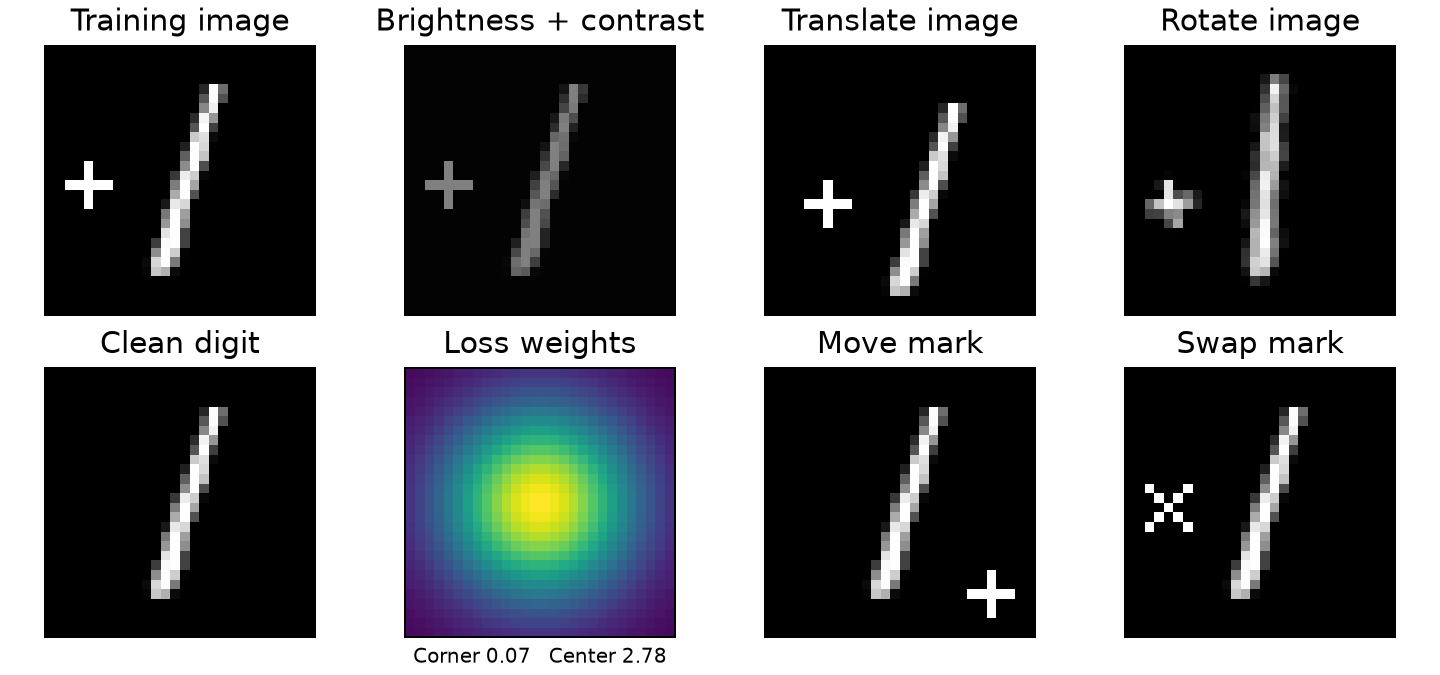
\includegraphics[width=.85\linewidth]{../figures/photometric.png}\end{center}
\smallcap{\textbf{Figure 1.} The same test digit throughout. The top row shows whole-image transformations of a fixed marked input. The bottom row shows the clean reference, the loss weights and two tests that change only the mark. Brighter yellow denotes a higher reconstruction weight. The model receives the ordinary grayscale image in the Gaussian condition.}

\sect{4 \quad Modifications to pretraining}
\textbf{Three augmentation policies.} Brightness and contrast jitter independently sample factors in $[0.7,1.3]$ and apply them in random order to each grayscale image [7]. Translation samples legal integer offsets of up to three pixels on each axis. Rotation samples legal angles from $0,\pm4,\pm8,\pm12$ degrees with bilinear interpolation. Spatial transforms move the entire digit and mark together. We check the image boundary before sampling so that moving the mark outside the crop cannot explain a gain. Every augmented view serves as both input and reconstruction target.

\textbf{Spatial prior.} For pixel $j$ at location $p_j$, the Gaussian replaces uniform MSE weights with $w_j\propto\exp[-\lVert p_j-(13.5,13.5)\rVert^2/(2\cdot7^2)]$, normalized to mean one. This fixed weighting uses the prior that the digit is centered. It adds no learned parameters. With ordinary augmentation the model still earns credit for reconstructing the transformed mark. Whether its clusters become less sensitive to that mark is an empirical question.

\newpage
\sect{5 \quad Ablation design and evaluation}
The marked training set has one fixed symbol per digit, with balanced random shape assignment independent of digit labels. Each of the three augmentation policies is crossed separately with Gaussian weighting on/off, sharing the ordinary and Gaussian-only controls. Four other arms train entirely on clean digits (ordinary, brightness/contrast, translation, rotation). This gives 12 arms and five matched seeds per arm. Each seed shares random initial weights, minibatch order, 12,000 training images, 100 pretraining epochs, architecture and optimizer. K-means with 20 restarts initializes each learned embedding. All arms then use ordinary IDEC on their unaugmented training images for 5,600 updates. The \href{https://github.com/JohnR31N/cs126FinalProj/blob/715521a/IDEC/photometric/design.md}{jitter protocol} and \href{https://github.com/JohnR31N/cs126FinalProj/blob/8e66ad4/IDEC/photometric/spatial_design.md}{spatial extension} specify the settings before their respective fits.

\textbf{Three distinct measurements.} Digit accuracy uses a cluster-to-digit mapping fitted on training labels after optimization and frozen for all 10,000 held-out digits. To measure sensitivity, move only the mark and count changes of cluster ID (primary). Then swap its shape at a fixed site. Finally fit a standardized logistic regression on the frozen final codes to read out plus versus cross. The probe sees both shapes on every training digit at the same site. Test it on both shapes for each unseen digit, with 50\% chance accuracy. Probe accuracy measures accessible shape information. A cluster can remain stable even when the representation retains that information.

\sect{6 \quad Results}
\begin{center}\small\setlength{\tabcolsep}{3pt}\begin{tabular}{lrrrrr}
\toprule
Pretraining & Marked ACC & Clean ACC & Move flips & Shape flips & Shape probe\\
\midrule
Ordinary IDEC & 67.51 & 70.22 & 6.23 & 5.36 & 50.20\\
Jitter only & 68.64 & 71.14 & 6.06 & 4.98 & 50.26\\
Translation & 80.63 & 81.61 & 3.41 & 2.73 & 50.21\\
Rotation & 74.01 & 76.08 & 5.05 & 4.00 & 50.15\\
Gaussian only & 71.42 & 73.47 & 5.19 & 4.53 & 50.13\\
\bottomrule
\end{tabular}
\end{center}
\smallcap{\textbf{Table 2.} Averages over five seeds, in percent. All rows train on marked images. Lower flip rates mean more stable assignments. The supplement includes all individual runs, joint arms, clean-training controls and paired differences.}
\begin{center}\small\setlength{\tabcolsep}{3pt}\begin{tabular}{lrrrr}
\toprule
Augmentation & Clean-only ACC & Clean-only gain & Joint marked ACC & Joint move flips\\
\midrule
Jitter only & 74.92 & $+1.39\pm2.29$ & 69.92 & 5.04\\
Translation & 83.87 & $+10.34\pm3.80$ & 79.93 & 3.66\\
Rotation & 82.41 & $+8.87\pm4.86$ & 76.32 & 4.05\\
\bottomrule
\end{tabular}
\end{center}
\smallcap{\textbf{Table 3.} The clean-only gain is the paired ACC difference in percentage points versus ordinary IDEC trained and tested without a mark (mean $\pm$ seed SD). Joint models train on marked images with that augmentation and Gaussian weighting.}
Brightness/contrast jitter increased mean marked accuracy by 1.13 percentage points. Its effect on movement flips was small (6.23\% to 6.06\%). In the mark-free controls it also improved mean clean accuracy, from 73.53\% to 74.92\%. Higher digit accuracy can therefore occur without exposure to the synthetic background feature. Gaussian weighting alone yielded 71.42\% marked accuracy and 5.19\% movement flips. The ordinary and jitter models both allowed a linear probe to classify the symbol at about chance.

Translation gave the strongest standalone result. Marked ACC rose by $13.12\pm2.98$ points and movement flips fell by $2.82\pm0.76$ points versus the matched baseline. It also raised ACC by $10.34\pm3.80$ points with no marks in training or testing. Both gains occurred in all five seeds. When those clean-trained models first encountered marks at test time, their movement flips averaged 11.69\% after translation training and 10.50\% without it. The clean accuracy gain alone therefore gives no guarantee of tolerance to an unfamiliar mark.

Adding Gaussian weighting to translation yielded 79.93\% marked ACC and 3.66\% movement flips, compared with 80.63\% and 3.41\% for translation alone. Gaussian weighting helped rotation on both outcomes. Across the five standalone conditions, the linear shape probe ranged from 50.13\% to 50.26\%, and all ten test clusters were occupied in every run.


\newpage
\sect{7 \quad Choice of solution and limits}
\textbf{Augmentation benchmark.} Compared within seed with Gaussian weighting alone, whole-image translation gained $9.21\pm2.42$ points of marked ACC and reduced movement flips by $1.78\pm0.30$ points. Both comparisons favored translation in all five seeds. Translation retains uniform reconstruction of every transformed pixel. Gaussian weighting directly changes the cost of errors according to their location.

An exploratory check compared exactly the clean digits that all five standalone models classified correctly within each seed (5,464--5,949 digits). On these shared examples, movement flips averaged 2.86\% for the baseline, 1.68\% for Gaussian weighting and 0.58\% for translation. This holds clean correctness fixed on a selected subset. The data still permit differences in cluster margins and in the information encoded in each representation.

\textbf{Sensitivity to centering.} We shifted each clean test digit four pixels horizontally and kept the 8,920 pairs for which every ink pixel stayed in frame. With the same trained model and label map, accuracy before and after displacement was 81.42\% and 29.46\% for translation, compared with 74.39\% and 10.09\% for Gaussian weighting. Translation transferred better to this shift, while all methods remained sensitive to substantially off-center handwriting. Method selection and evaluation used these same held-out digits, so the ranking needs a separate dataset to establish transfer.


\textbf{What the tests establish.} Moving only the background mark identifies its effect on that frozen model's cluster assignment for these image pairs. Mark-free training and testing can reveal a benefit even when no synthetic symbol is present. Both effects may coexist. These comparisons do not estimate what fraction of a change in ACC is mediated by suppressing the background. A linear readout covers one shape contrast. Nonlinear features, position information and other backgrounds may behave differently.

Boundary checks also affect the amount of augmentation. On marked images an average of 31.7 of the 49 possible translations fit, versus 45.5 on clean images. Rotation kept the original orientation with expected probability 25.5\% on marked images and 14.6\% on clean images. These differences matter when comparing gains between the two domains.

\textbf{Relation to the preceding study.} An earlier experiment explicitly moved or replaced the mark during pretraining. That targeted augmentation gave 4.34\% movement flips, versus 6.20\% for its fixed-input baseline. A paired reconstruction target [6] further reduced the decoder's response to mark movement but had mixed effects on assignment stability. The current augmentation comparison holds the assigned symbol fixed relative to the handwriting and tests conventional transforms. The earlier \href{https://github.com/JohnR31N/cs126FinalProj/tree/idec-final-v1.5/IDEC}{report, predictions and code} remain available with their own protocol.
